\documentclass[11pt]{article}
\usepackage[a4paper,margin=27mm]{geometry}
\usepackage{amsmath,amssymb,amsthm,booktabs,longtable,array}
\usepackage[T1]{fontenc}
\usepackage{lmodern}
\usepackage{graphicx}
\usepackage[hidelinks]{hyperref}
\newtheorem{theorem}{Theorem}[section]
\newtheorem{lemma}[theorem]{Lemma}
\newtheorem{proposition}[theorem]{Proposition}
\newtheorem{remark}[theorem]{Remark}
\newcommand{\R}{\mathbb R}
\newcommand{\sgn}{\operatorname{sgn}}
\newcommand{\stick}{\operatorname{stick}}
\newcommand{\code}[1]{\nolinkurl{#1}}
\setlength{\emergencystretch}{2em}
\title{The stick number of $8_1$:\\a computer-assisted proof with a partially formalized geometric reduction}
\author{Griffith Wang\\[3pt]\small\href{mailto:griffithgwang@gmail.com}{\texttt{griffithgwang@gmail.com}}}
\date{Draft of September 10, 2026}
\begin{document}
\maketitle
\begin{abstract}
We present a computer-assisted argument that the Rolfsen knot $8_1$ has
stick number ten. An exposed-vertex projective construction associates to
every hypothetical nine-stick representative a diagram with eight shadow
edges, one of which passes over every crossing. Necessary determinant-sign,
height-compatibility, blocked-ear, and diagram-invariant conditions give a
Boolean formula on 142 geometric signs. Its explicit gate encoding has
18,597 variables and 76,298 clauses and is refuted by a fixed LRAT
certificate. Lean 4 verifies this fixed refutation, the source-to-CNF
translation, and the real-geometric validity of 2,283 of the 2,294 source
constraints. The remaining nine ear conditions and two invariant conditions,
as well as the global topological reduction, are justified in ordinary
mathematics and are explicitly outside the formalized theorem. An exact
rational ten-gon and a checked Reidemeister trace provide a separate upper
bound. We describe the certificate interfaces and trust boundary so that
the computation and its geometric interpretation can be reviewed separately.
\end{abstract}

\section{Statement and proof architecture}
The stick number $\stick(K)$ of a tame knot $K$ is the least number of
straight segments in an embedded polygon representing $K$ in $\R^3$.
Lengths are unrestricted; this is not the equilateral stick number.
Mirroring a polygon preserves its number of edges.

\begin{theorem}\label{thm:main}
The Rolfsen knot $8_1$ satisfies $\stick(8_1)=10$.
\end{theorem}

Calvo's classification of octagonal knots \cite[Theorem 1(iv)]{calvo}
excludes $8_1$ and its mirror, and hence gives $\stick(8_1)\geq9$.
Subdividing edges explains why the same classification excludes every
smaller polygon. The construction of Huh, No, and Oh
\cite[Theorem 1.1]{hno} gives $\stick(K)\leq c(K)+2$ for a two-bridge knot
of crossing number at least six. It therefore gives the upper bound ten
for $8_1$. We also supply an independent exact upper-bound certificate.
Neither external theorem supplies the nine-stick exclusion proved here.
We make no claim that the present work is a classification of all nine-stick knots.

The lower-bound argument uses only necessary conditions. In particular,
we never assert that every satisfying abstract sign assignment is realizable
by points in $\R^3$. An unsatisfiable relaxation suffices: a geometric
counterexample would induce a satisfying assignment, whereas the fixed
formula admits none. The eleven source conditions not yet derived from
geometry inside Lean are mathematical obligations, not omitted clauses
of the finite formula. All 2,294 clauses at the source level participate
in the certified exclusion.

The argument has three distinct layers:
\begin{enumerate}
\item Ordinary geometry and knot theory put any counterexample into a
positive, nondegenerate projective frame and identify its diagram invariants.
\item Real-algebraic Lean proofs establish the determinant and order
conditions of this frame. A conditional formal theorem exposes precisely
the eleven remaining source-root premises.
\item A formal source-to-circuit-to-CNF translation and an accepted LRAT
refutation exclude the finite conjunction.
\end{enumerate}
The conclusion is a computer-assisted theorem with partial formalization,
not an end-to-end Lean theorem about ambient-isotopy classes of knots.

\section{The exposed-vertex construction}\label{sec:roof}
Write a hypothetical embedded nine-gon in cyclic order as
$p_0,\ldots,p_7,v$. Embeddedness and knot type are stable under sufficiently
small perturbations of its vertices. Here is an explicit ambient extension
which avoids any assumption about extending arbitrary topological isotopies.
Triangulate a large cube compatibly with the polygon, allowing subdivision
of its edges. Prescribe a displacement at each original polygon vertex,
interpolate it linearly along polygon edges, set it to zero at all other
triangulation vertices, and extend affinely on each simplex. The resulting
continuous displacement $u$ vanishes on the cube boundary; extend it by
zero outside. Since the triangulation is finite, sufficiently small vertex
displacements make the global Lipschitz constant $L$ of $u$ less than one.
Then $H_t(x)=x+t u(x)$ is an ambient isotopy: injectivity follows from
\[
 |H_t(x)-H_t(y)|\geq(1-tL)|x-y|,
\]
and surjectivity follows by applying the contraction principle to
$x\mapsto y-t u(x)$ for each $y$. The inverses are jointly continuous
by the same uniform estimate. Each polygon edge is mapped linearly onto
the corresponding perturbed edge. This proves both embeddedness and knot
preservation for sufficiently small vertex perturbations. This finite
triangulation argument is ordinary mathematics, not a Lean theorem here.

Choose a vertex $v$ exposed by a supporting linear functional. After an
affine coordinate change, $v=0$ and
$p_i=(x_i,y_i,z_i)$ with $z_i>0$. Put
\[
 q_i=(x_i/z_i,y_i/z_i),\qquad h_i=1/z_i,\qquad P_i=(q_i,h_i).
\]
Here and below shadow indices are taken modulo eight.

\begin{lemma}[Roof diagram]\label{lem:roof}
The polygon has a diagram, up to mirror image, consisting of the projected
chain $q_0q_1\cdots q_7$ closed by $q_7q_0$. Crossings among chain edges
use the affine heights $h_i$. At every crossing involving the closing
shadow edge, that edge is the overpassing strand. The closing edge
represents two spatial segments.
\end{lemma}
\begin{proof}
On the open half-space $z>0$ the projective map
$F(x,y,z)=(x/z,y/z,1/z)$ is a diffeomorphism and maps segments to segments.
To check its effect on knot type, set
\[
 d_\theta=\cos\theta+z\sin\theta,\qquad
 G_\theta(x,y,z)=\left(\frac{x}{d_\theta},\frac{y}{d_\theta},
 \frac{z\cos\theta-\sin\theta}{d_\theta}\right),
 \quad 0\leq\theta\leq\frac\pi2.
\]
The denominator is positive and the projective transformation is
invertible on its image. Segments remain segments, so for a compact
polygon in this half-space these maps give a continuous path of embedded
polygons from the identity to $F$ followed by reflection in the last
coordinate. Along this path the knot type is locally constant by the
small-perturbation construction above; compactness of the parameter
interval gives a finite concatenation of its ambient isotopies.
This justifies ``up to mirror image'' without inferring knot equivalence
merely from an arbitrary diffeomorphism of an open set.

Choose $r$ in the interior of $q_7q_0$, away from all its crossings.
Replace $v$ by $\varepsilon(r_x,r_y,1)$ with $\varepsilon>0$ sufficiently
small. Stability preserves the knot type. Its image under $F$ is
$(r,1/\varepsilon)$. The two incident projected segments subdivide
$q_7q_0$. At each of its finitely many crossings with the chain, the
coefficient of $1/\varepsilon$ in the interpolated height is strictly
positive. Thus all these heights eventually exceed the chain height.
The two pieces have the same oriented shadow direction, so the
subdivision introduces no diagram crossing.
\end{proof}

We choose the initial polygon generically so that every determinant used
below is nonzero: all four-point spatial volumes, all three-point shadow
orientations, and all three-line shadow brackets. These conditions are
compatible with the exposed vertex and with knot preservation.
The coordinates $(q_i,h_i)$ vary in an open set with $h_i>0$.
Each prohibited determinant is a nonzero polynomial in these coordinates.
For spatial volumes and planar orientations this follows by freely
moving one of the involved points. Three pairwise nonadjacent shadow
lines can be chosen independently, so their concurrency determinant
is not identically zero. If an adjacent pair occurs, the factorization
in Section~\ref{sec:signs} reduces the assertion to nonzero orientation
polynomials. A finite union of proper polynomial zero sets has empty
interior. It can therefore be avoided in the open set of admissible
perturbations. In particular, no exceptional coordinate family is
silently excluded from the universal nine-gon argument.

\section{Signs and necessary algebraic constraints}\label{sec:signs}
Use homogeneous columns
\[
 w_i=(q_{ix},q_{iy},h_i,1)\ (0\leq i<8),\qquad w_8=(0,0,1,0).
\]
Our alternating sign convention is
$\chi(i,j,k,l)=\sgn(-\det(w_i,w_j,w_k,w_l))$.
For finite indices this is the sign of
\[
 V(i,j,k,l)=\det(P_j-P_i,P_k-P_i,P_l-P_i),
\]
and $\chi(i,j,k,8)=\sgn T(i,j,k)$, where
$T(i,j,k)=\det(q_j-q_i,q_k-q_i)$.
Reflecting the first planar coordinate if necessary makes $T(0,1,2)>0$.
The corresponding mirror has the same crossing number and $a_2$.

There are $\binom94=126$ independent sorted point signs. For shadow edge
$i$ set $u_i=q_{i+1}-q_i$ and
\[
 L_i=(-u_{iy},u_{ix},\det(q_i,u_i)),\qquad
 C(i,j,k)=\det(L_i,L_j,L_k).
\]
Here $L_i\cdot(x,y,1)=0$ is its supporting line. Of the triples of
shadow edges, sixteen have no adjacent pair. Their bracket signs are
additional Boolean inputs. If $b=a+1$ modulo eight, direct expansion gives
\begin{equation}\label{eq:adjacent}
 C(i,a,b)=T(i,i+1,b)T(a,b,b+1).
\end{equation}
Alternation supplies every other order of the indices. Thus only 142
geometric Boolean inputs are needed. Positive signs are encoded as true;
negation changes the sign, and Boolean equality multiplies two signs.

The three-term Grassmann--Pluecker identities imply that their three
signed nonzero products cannot all have the same sign. Apply these
identities to rank-four point brackets and rank-three line brackets.
There are respectively 1,260 and 280 resulting conditions. The relation
\begin{equation}\label{eq:bracket}
 C(ab,cd,ef)=T(a,b,e)T(c,d,f)-T(a,b,f)T(c,d,e)
\end{equation}
gives 48 additional mixed-sign conditions. Consistency of the adjacent
factorization gives another 48.

The columns $w_i$ have a common strictly positive functional: their
third coordinate is $h_i>0$ for finite $i$ and one for $i=8$.
For any five columns, their alternating four-minor dependence has
coefficients of both signs; otherwise applying this functional gives
a nonzero quantity of one sign equal to zero. The analogous statement
for $(q_{ix},q_{iy},1)$ uses the last-coordinate functional. These give
126 homogeneous and 70 projected acyclicity conditions. Normalization
adds one condition. All these are necessary properties of real points;
no converse realizability theorem is used.

\section{Height compatibility}
Only edges $0,\ldots,6$ are finite spatial lines. For each choose an
affine function $F_i(x,y)$ taking the required endpoint heights, and
write $F_i$ also for its coefficient vector. Such a function exists
because projected endpoints are distinct. Define
\[
 H_{ij}=V(i,i+1,j,j+1)
       =(F_i-F_j)\cdot(L_i\times L_j).
\]
The second equality is a determinant identity. It is independent of the
arbitrary extension of the height function away from its line.
For adjacent indices $H_{ij}=0$; for nonadjacent finite edges it is nonzero.

\begin{lemma}[Height stresses]\label{lem:stress}
If $\sum_i\lambda_iL_i=0$, then
\begin{equation}\label{eq:stress}
 \sum_{i<j}\lambda_i\lambda_jH_{ij}=0.
\end{equation}
More generally, if a symmetric matrix $\Omega$ satisfies
$\sum_j\Omega_{ij}L_j=0$ for every $i$, then
$\sum_{i<j}\Omega_{ij}H_{ij}=0$.
\end{lemma}
\begin{proof}
In the latter sum the coefficient paired with $F_i$ is
$\sum_{j\ne i}\Omega_{ij}(L_i\times L_j)
=L_i\times\sum_j\Omega_{ij}L_j=0$.
Taking $\Omega_{ij}=\lambda_i\lambda_j$ proves the first assertion.
\end{proof}

For each four-subset of the seven finite lines, use the alternating
three-minor dependence for $\lambda$. Remove terms with adjacent edges
and translate the remaining zero sum into the requirement that its
nonzero terms have both signs. This supplies $\binom74=35$ conditions.

A useful strengthening comes from five lines in order $(h,a,b,c,d)$.
Let the dependence on $(h,a,b,c)$ be
\[
 v=(C(a,b,c),-C(h,b,c),C(h,a,c),-C(h,a,b),0)
\]
and the dependence on $(h,a,b,d)$ be
\[
 w=(C(a,b,d),-C(h,b,d),C(h,a,d),0,-C(h,a,b)).
\]
Define $\Omega=w_aw_bvv^{\mathsf T}-v_av_bww^{\mathsf T}$.
It satisfies the lemma; its off-diagonal entries at $ab$ and $cd$
vanish. The remaining eight coefficients factor as
\begin{align*}
 \Omega_{ha}&=-v_aw_a C(h,a,b)C(a,c,d),\\
 \Omega_{hb}&= v_bw_b C(h,a,b)C(b,c,d),\\
 \Omega_{ic}&=w_aw_bv_iv_c\quad(i=h,a,b),\\
 \Omega_{id}&=-v_av_bw_iw_d\quad(i=h,a,b).
\end{align*}
These factorizations follow from the same three-term bracket identity
and are also proved over $\R$ in Lean. Their factors are all nonzero.
Deleting adjacent-edge terms again leaves a mixed-sign zero sum.
For each five-subset choose one of five hubs and one of three pairings
of the other four lines. The resulting $\binom75\cdot5\cdot3=315$
conditions are the five-line height constraints.

None of these height stresses is imposed on the overpassing closing
shadow edge. Giving that edge an affine height would change the class
of spatial polygons and invalidate the reduction.

\section{The nine blocked-ear conditions}\label{sec:ears}
For an embedded polygon in general position, an ear at a vertex is the
closed triangle spanned by that vertex and its two neighbours.

\begin{lemma}\label{lem:ear}
Every ear of a nine-stick $8_1$ is pierced through its relative interior
by an edge whose endpoints are not vertices of that triangle.
\end{lemma}
\begin{proof}
If no such edge pierces the triangle, slide the two incident sides
across its disk onto the third side and remove the redundant vertex.
More explicitly, move the middle vertex linearly toward an interior
point of the third side. This gives a path of embedded nine-gons ending
at a subdivision of the eight-gon; the small-perturbation argument of
Section~\ref{sec:roof}, applied along the parameter interval, preserves
ambient knot type. General
position rules out boundary intersections: a nonincident edge meeting
a triangle side would make four vertices coplanar, and an edge incident
to a triangle vertex leaves its plane immediately. The disk's interior
is otherwise disjoint from the knot by hypothesis. The resulting
eight-edge polygon represents the same knot, contrary to Calvo's
classification. Of the nine polygon edges, exactly five avoid all
three vertices of a given ear, so these are precisely the eligible edges.
\end{proof}

For distinct vertices $a,b,c,s,t$ the piercing condition is
\begin{align}
 V(a,b,c,s)V(a,b,c,t)&<0,\label{eq:pierce1}\\
 V(s,t,a,b)V(s,t,b,c)&>0,\label{eq:pierce2}\\
 V(s,t,a,b)V(s,t,c,a)&>0.\label{eq:pierce3}
\end{align}
To verify it, intersect the segment's line with the triangle plane.
Equation~\eqref{eq:pierce1} places the unique intersection strictly
between $s$ and $t$. Cramer's rule expresses its three barycentric
coordinates as a common nonzero factor times the three quantities in
\eqref{eq:pierce2}--\eqref{eq:pierce3}. They are all strictly positive
after normalization exactly when those quantities have the same sign.
This proves both directions, including the strict-interior requirement.

One must also justify the use of index eight, which denotes an ideal
point rather than a finite vertex. Before the apex perturbation in
Lemma~\ref{lem:roof}, apply the invertible homogeneous linear map
\[
 (x,y,z,t)\longmapsto(x,y,t,z)
\]
to the original polygon. Divide finite columns by their positive $z_i$;
the original apex $(0,0,0,1)$ becomes $w_8$ without a negative rescaling.
Every four-minor is multiplied by the same determinant sign and by
positive factors. The products and sign equalities in the piercing
test are consequently unchanged. Thus the nine blocked-ear disjunctions
are inherited from the original polygon, including the three ears
involving the apex. No Euclidean triangle with a vertex at infinity
is being assumed without this homogeneous justification.

These nine conditions are at source indices $2183,\ldots,2191$
(zero-based). Their Boolean expression and gate translation are
certified, but Lemma~\ref{lem:ear} and its link to these expressions
remain outside the present Lean proof.

\section{Diagram extraction and the Conway coefficient}\label{sec:diagram}
There are twenty pairs of nonadjacent shadow edges. For such a pair
$(i,j)$, their open segments cross precisely when
\begin{align*}
 T(i,i+1,j)T(i,i+1,j+1)&<0,\\
 T(j,j+1,i)T(j,j+1,i+1)&<0.
\end{align*}
These strict segment-intersection conditions have been proved in Lean
using Cramer's rule. At a crossing put $D_{ij}=\det(u_i,u_j)$.
The intersection parameters lie in $(0,1)$ and
\[
 \sgn D_{ij}=\sgn T(i,i+1,j+1),\qquad D_{ji}=-D_{ij}.
\]
For two finite chain edges the height of edge $i$ minus that of edge
$j$ is $H_{ij}/D_{ij}$. Adopt the crossing-sign convention in which
an overpassing first edge contributes $\sgn D_{ij}$.
The crossing sign is therefore $\sgn H_{ij}$ and the first visit is
under precisely when this differs from $\sgn D_{ij}$.
For a crossing with edge seven, the first edge is always under;
its crossing sign is $-\sgn D_{i7}$. Reversing all crossing signs
would not affect the pair products below, but the code uses this
single convention consistently.

For two live crossings on edge $i$, solving the line intersections gives
\begin{equation}\label{eq:order}
 t_{ij}-t_{ik}=-\frac{C(i,j,k)}{D_{ij}D_{ik}}.
\end{equation}
The nonconcurrency hypothesis makes the difference nonzero. Along a
fixed edge, the earlier event is thus determined by the sign of
$C(i,j,k)D_{ij}D_{ik}$. Events on different edges follow their cyclic
edge order, with the basepoint at $q_0$. This determines the complete
Gauss traversal from the sign assignment. The formula explicitly
includes twenty conditional direction relations and eighty conditional
three-event transitivity relations. Their geometric validity, including
the live-crossing guards, is proved in \code{DirectionRoots.lean} and
\code{OrderRoots.lean}.

Write $\nabla_K(z)=1+a_2(K)z^2+\cdots$ for the Conway polynomial,
normalized by $\nabla_{\mathrm{unknot}}=1$ and
$\nabla_{K_+}-\nabla_{K_-}=z\nabla_{L_0}$.
For a crossing $c$, let $\epsilon_c\in\{-1,1\}$ be its sign and let
$U_c$ record whether its first visit in the based traversal is under.
Two crossings are interleaved if exactly one endpoint of one Gauss
chord lies between the endpoints of the other.

\begin{lemma}[Based pair formula]\label{lem:a2}
For any regular based knot diagram,
\begin{equation}\label{eq:a2}
 2a_2(K)=\sum_{\{c,d\}\text{ interleaved},\ U_c\ne U_d}
                \epsilon_c\epsilon_d.
\end{equation}
\end{lemma}
\begin{proof}
Switch the crossings with $U_c=1$, in the order of their first visits.
The final diagram is descending and represents the unknot. The skein
relation says that the change at $c$ is $\epsilon_c$ times the linking
number of its oriented smoothing. Twice that linking number is the
sum of the current signs of crossings between the two smoothing
components. These are exactly the chords interleaved with $c$.

Consider one interleaved unordered pair. If neither crossing is switched
there is no contribution. If only one is switched, its contribution to
twice the total change is the original product
$\epsilon_c\epsilon_d$. If both are switched, the contribution when the
first is switched uses the original sign of the second; when the second
is switched it uses the reversed sign of the first. The two cancel.
Summing and using $a_2(\mathrm{unknot})=0$ proves the formula. In
particular the formula does not require a crossing-minimal diagram.
\end{proof}

The knot $8_1$ has crossing number eight and Conway polynomial
$1-3z^2$ \cite{katlas}. The latter value is also recovered exactly from the identified
ten-gon diagram in Section~\ref{sec:upper}. Consequently its roof
diagram, or a mirror diagram, satisfies
\[
 \sum_c [c\text{ is live}]\geq8,\qquad
 \sum_{\{c,d\}\text{ interleaved},\ U_c\ne U_d}
                 \epsilon_c\epsilon_d=-6.
\]
These are the last two source constraints. The implementation tests
interleaving by comparing the two visits of one crossing with the
open interval between the visits of the other, uses inequality of the
first-under flags, and adds $+1$ or $-1$ according to equality of the
crossing signs. Inactive crossing pairs contribute zero. Thus its
pseudo-Boolean sums are exactly the quantities displayed above.

The counter circuitry implementing these sums is proved correct in
Lean for arbitrary boundary values. The interpretation as $a_2$ and
the knot-theoretic lower bound on diagram crossings are external
mathematical inputs; they are not consequences merely of counter correctness.

\section{The finite refutation and its formal interface}\label{sec:formal}
The base call \code{roof_boolean.build()} constructs the conjunction
in Table~\ref{tab:roots}. All optional strengthening flags are false:
there is no canonical labelling, chord condition, Fox-colouring condition,
or additional endpoint simplification in the certified formula.

\begin{table}[ht]
\centering\small
\begin{tabular}{lrrl}
\toprule
Source family & Start & Count & Geometric Lean link\\
\midrule
Point Pluecker &0&1260&proved\\
Line Pluecker &1260&280&proved\\
Line brackets &1540&48&proved\\
Homogeneous acyclicity &1588&126&proved\\
Projected acyclicity &1714&70&proved\\
Normalization &1784&1&proved\\
Line incidence &1785&48&proved\\
Four-line heights &1833&35&proved\\
Five-line heights &1868&315&proved\\
Blocked ears &2183&9&external\\
Crossing directions &2192&20&proved\\
Event transitivity &2212&80&proved\\
Conway target &2292&1&external\\
Crossing target &2293&1&external\\
\bottomrule
\end{tabular}
\caption{Zero-based source-root slices. ``External'' concerns geometric
interpretation; every row has a certified Boolean-to-CNF translation.}
\label{tab:roots}
\end{table}

The source is a 23,565-node acyclic expression graph. Its 23,563 ordinary
Boolean nodes and two pseudo-Boolean nodes are connected to an explicit
circuit of 18,454 gates. The gates are AND, Boolean equivalence, and
majority; full adders and balanced counters are built from them.
An additional constant variable gives 18,597 CNF variables in total.
The roots include the 2,294 source conditions and the true constant.
Each gate receives its defining equivalence clauses, and each root
receives a unit clause. The resulting CNF has 76,298 clauses.

For a well-ordered gate list, an assignment to the inputs extends by
evaluation to every gate. The defining clauses hold under this
extension; root unit clauses hold exactly when their circuit outputs
are true. Lean proves this fact for arbitrary such circuits. Local
exhaustive checks connect each ordinary source operation to its gate
implementation. For the actual counter circuits, bit-vector proofs
establish equality and threshold semantics with sufficient widths to
exclude overflow. Signed weights are normalized using
$-b=(1-b)-1$ for a Boolean value $b\in\{0,1\}$.
The actual gate-generated CNF is proved equal to the fixed CNF after
semantics-preserving clause and literal normalization.

The fixed CNF was refuted by CaDiCaL. An independent DRAT checker
produced an LRAT certificate, which was also accepted by a C LRAT
checker. Clause identifiers were densely renumbered, preserving
clauses and hints, for the Lean checker. The resulting proof has
1,577,701 actions. Its dense textual form is 700,460,899 bytes.
The authoritative byte hashes are
\begingroup\footnotesize
\begin{verbatim}
b7034c3c955b2cf9c3a7878439f25941c0f51c5eeebb421b727d2ebfd2227f7c
97d9c4224e353ea24ac09b5373be1fb217d2ef057577cb6f01b6475b05190a87
\end{verbatim}
\endgroup
The first line is the CNF hash and the second is the dense LRAT hash.

\code{FixedCertificate.lean} embeds the CNF and compressed proof bytes
as fixed constants, decompresses and parses them through pure functions,
and proves checker acceptance by \code{native_decide}. It then applies
Lean's standard \code{LRAT.check_sound} to obtain
\code{Stick81.roofUnsat}. There is no acceptance hypothesis in this
theorem. A program that only reads files and prints ``true'' would not,
by itself, be this fixed-input theorem.

\begin{proposition}[Formal finite exclusion]\label{prop:formal}
For the fixed source graph, no assignment satisfying its node semantics
and its true constant makes all 2,294 source roots true. Moreover,
for a positive nondegenerate normalized real frame, it suffices to
assume the nine ear roots and the two target roots true to obtain a
contradiction.
\end{proposition}
\begin{proof}
The first assertion is \code{Stick81.source_formula_unsat}.\par
For the second, the algebraic, direction, and order lemmas supply 2,283
roots. The checked partition and eleven premises give all roots, so the
first assertion applies. The resulting Lean theorem is named
\code{geometric_exclusion_eleven} in namespace \code{Stick81.Submission}.
\end{proof}

The geometric frame in this statement is actual real coordinate data,
not an uninterpreted name for an arbitrary Boolean assignment.
Its genericity, positive heights, and normalization are explicit
hypotheses. The source-model hypothesis specifies evaluation of the
acyclic source graph at the frame's determinant signs. Such evaluation
exists by recursion in source order; it is not a satisfiability
assumption about its roots. In applying the proposition to a polygon,
this recursive evaluation is the intended assignment.

\section{Exact upper bound and final assembly}\label{sec:upper}
The file \code{known_10gon.tab} specifies ten triples of finite decimals.
Every decimal is read as its exact rational value. The independent
arithmetic checker \code{exact_polygon.py} examines all 35 pairs of
nonadjacent edges and validates a regular projection with eighteen
crossings, including intersection parameters and nonzero height
differences. Adjacent edges are nondegenerate with distinct directions.
These checks certify an embedded ten-gon, not its knot type alone.

\begin{figure}[ht]
\centering
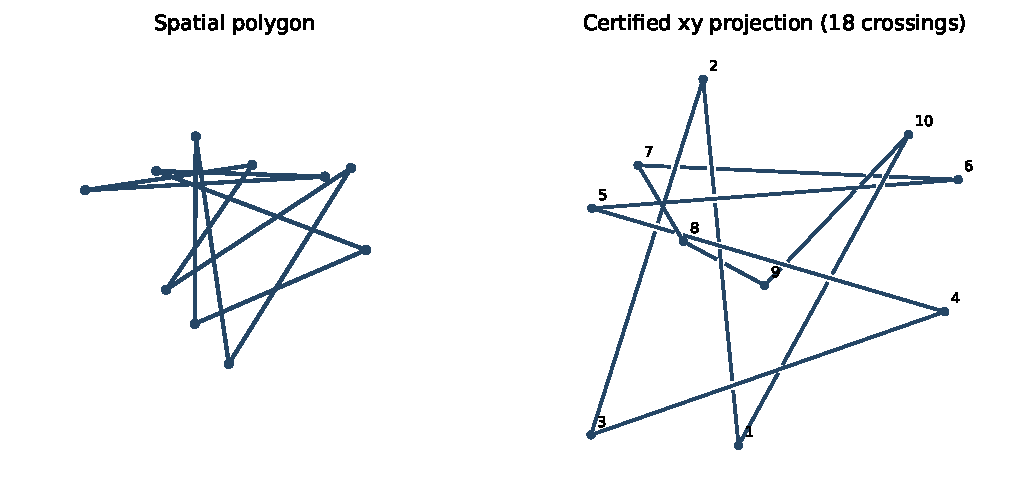
\includegraphics[width=\linewidth]{tengon.pdf}
\caption{The rational ten-gon: a spatial illustration (left) and its
certified projection (right). Vertices in this figure are numbered
one through ten in file order. Underpass gaps on the right come from
the exact crossing certificate. Floating-point coordinates are used
only to draw the figure, not to verify the polygon.}
\label{fig:tengon}
\end{figure}

The file \code{reidemeister_proposed.json} supplies thirty local moves.
The standard-library checker \code{check_reidemeister.py} verifies
each move on a four-valent rotation system with over/under parity:
monogon or cancellable bigon removal for types I and II, and an empty
triangular-face rewiring with consistent height order for type III.
It checks continuity of the trace and a final orientation-preserving,
over/under-preserving dart isomorphism to the PD code
\begin{verbatim}
[[1,9,2,8],[3,7,4,6],[5,12,6,13],[7,3,8,2],
 [9,1,10,16],[11,15,12,14],[13,4,14,5],[15,11,16,10]]
\end{verbatim}
This is also matched to Spherogram's named $8_1$ table entry
\cite{spherogram}. Thus identification is based on a diagram equivalence
trace, not on equality of a polynomial. The upper-bound computation is
independent of the lower-bound SAT search and is not presently formalized
as an ambient-isotopy theorem in Lean. The published two-bridge upper
bound provides a second route to the same inequality.

\begin{samepage}
\begin{proof}[Proof of Theorem~\ref{thm:main}]
Suppose that a nine-edge representative exists. Section~\ref{sec:roof}
gives a positive generic normalized frame and a roof diagram of the knot
or its mirror. Sections~\ref{sec:signs}--\ref{sec:diagram} show that its
determinant signs satisfy all source constraints: the ordinary
geometric lemmas supply the nine ears and two targets, and the real
algebraic conditions supply the other 2,283. Evaluate the source graph
at these signs and apply Proposition~\ref{prop:formal} to obtain a
contradiction. Thus no nine-edge representative exists. Calvo's
classification excludes all smaller edge counts, and either upper-bound
argument above gives ten edges. Therefore the minimum is ten.
\end{proof}

\end{samepage}
\section{Trust boundary, reproduction, and limitations}
The pinned versions are Lean 4.19.0 and mathlib commit
\begin{verbatim}
c44e0c8ee63ca166450922a373c7409c5d26b00b
\end{verbatim}
The audited final theorem depends on
\code{propext}, \code{Classical.choice}, \code{Quot.sound}, and
\code{Lean.ofReduceBool}. The last is the native-reflection trust
boundary: the Lean compiler and runtime used for native computation
are trusted in addition to the ordinary proof-checking machinery.
There is no \code{sorryAx} in this theorem's audited dependency list
and no new axiom asserting the knot theorem or the eleven missing
geometric implications. Solver heuristics and the compression program
are not trusted to establish unsatisfiability: their output must pass
the certified checker.

The ratio $2283/2294$ is an inventory of source roots, not a probability
of correctness or a measure of mathematical difficulty. One incorrectly
justified necessary condition could invalidate the nine-gon exclusion.
Conversely, an ordinary mathematical proof need not be written in Lean
to be valid. The essential remaining review tasks are the global
coverage argument, the ear-collapse and homogeneous-piercing argument,
and the interpretation of the diagram selectors and Conway sum.

Exact rational controls, comparison with an independently calculated
Alexander coefficient, and independent certificate replays are useful
diagnostics. They are not substitutes for the universal implications.
In particular, random examples do not prove that all geometric inputs
are covered. The formalized topology definitions in the development
are not yet connected to a theorem \code{stick(K81) = 10}.

The public source repository is
\begin{center}\small
\url{https://github.com/griffithwang/stick8-1-certificate}.
\end{center}
The verified audit release is pinned to commit
\begin{verbatim}
0b88e7c65ab01fbe281920946d58ae079191ec39
\end{verbatim}
It contains the source dependency closure, pinned build instructions,
finite data, and a hash manifest. Large certificates are separate
release assets rather than ordinary Git objects. Use the fixed audit release
\code{v0.1.0-audit} for the certificates and machine-readable verification
record. All 59 local Lean modules were rebuilt successfully on Windows;
upstream mathlib dependencies used a pinned cache. Per-module source hashes,
exit codes, and timings are recorded separately from the independent
arithmetic and C-checker replays. This is not a claim of a clean build on
every platform.

\paragraph{Use of generative AI.}
Generative AI tools, including OpenAI Codex, were used extensively in
developing and reviewing mathematical arguments, implementing the
computational and Lean components, and drafting this manuscript.
The scope and limitations of formal verification are stated explicitly.
The author assumes responsibility for the submitted work, including its
mathematical claims, code, and references. AI-assisted review is not
independent human peer review.

\paragraph{License.}
The manuscript and original figures are licensed under
\href{https://creativecommons.org/licenses/by/4.0/}{CC BY 4.0}.
The original accompanying code is available under the MIT License;
third-party components retain their existing licenses.

\begin{thebibliography}{9}
\bibitem{calvo} J. A. Calvo,
\emph{Geometric Knot Spaces and Polygonal Isotopy},
\href{https://arxiv.org/abs/math/9904037v2}{arXiv:math/9904037v2} (1999),
Theorem 1(iv).
\bibitem{hno} Y. Huh, S. No, and S. Oh,
\emph{Stick numbers of $2$-bridge knots and links},
\href{https://arxiv.org/abs/1411.1850}{arXiv:1411.1850} (2014),
Theorem 1.1.
\bibitem{spherogram} The Spherogram developers,
\emph{Spherogram}, version 2.4.1, named knot table and planar diagrams,
\url{https://github.com/3-manifolds/Spherogram}.
\bibitem{lean} The Lean developers,
\emph{Lean 4}, version 4.19.0, standard LRAT checker and soundness theorem,
\url{https://github.com/leanprover/lean4/tree/v4.19.0/src/Std/Tactic/BVDecide/LRAT}.
\bibitem{katlas} D. Bar-Natan and S. Morrison (eds.),
\emph{The Knot Atlas}, entry $8_1$, polynomial data,
\url{https://katlas.org/wiki/8_1}, accessed September 10, 2026.
\end{thebibliography}
\end{document}
